\clearpage
{\hspace{-5.5mm}\Huge Reading Guide}

We have structured the report as a variant of IMRAD, adapted to engineering
projects. It follows the V-model, as shown in
\autoref{fig:v-model-report-structure}, with the academic parts added:
\textit{Introduction}, \textit{Method}, \textit{Discussion} and
\textit{Conclusion}.

% ------------------------------------------------------------
% EXAMPLE of a DrawIO figure:
% The source file is assets/drawio/v-model.drawio - latexmk converts
% it to assets/drawio/v-model.pdf automatically before compiling.
% ------------------------------------------------------------
\begin{figure}[H]
  \centering
    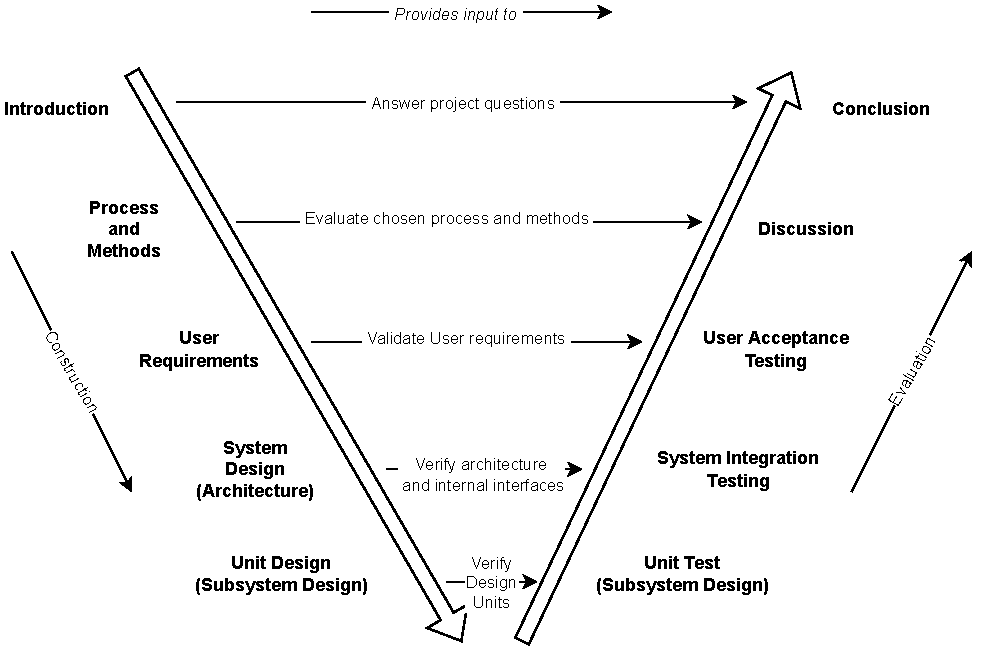
\includegraphics[width=\linewidth]{assets/drawio/v-model.pdf}
    \caption{Report structure based on the V-model. Each chapter on the left is checked by the chapter at the same level on the right, e.g. the acceptance test validates the user requirements.}
    \label{fig:v-model-report-structure}
\end{figure}

In broad terms the report describes the project from idea, through
requirements, to architecture, design, test and evaluation.

